% Gabarit pandoc des corrigés publiés (brut et guidé). Contenu sans marque ni nom de site.
% Compilation : lualatex (latexmk -lualatex).
% Le Markdown reste la source unique : ne pas éditer ce fichier .tex à la main.
\documentclass[11pt,a4paper]{article}

% --- Moteur, polices (Latin Modern) et langue ---------------------------------
\usepackage{iftex}
\ifLuaTeX\else\errmessage{Ce document se compile avec lualatex}\fi
\usepackage{amsmath,amssymb,mathtools}
\usepackage{fontspec}
% mathrm=sym : \mathrm prend ses glyphes dans la police mathématique (ℓ, μ, Ω), comme KaTeX.
\usepackage[math-style=TeX,bold-style=TeX,mathrm=sym]{unicode-math}
% Repli pour les glyphes absents de Latin Modern (indices et exposants Unicode,
% flèches, filets des schémas en texte, symboles) : DejaVu, puis Latin Modern Math
% (ℓ, lettres mathématiques Unicode des légendes).
\directlua{
  luaotfload.add_fallback("repliTexte", {"DejaVuSerif:mode=harf;", "DejaVuSans:mode=harf;", "file:latinmodern-math.otf:mode=harf;"})
  luaotfload.add_fallback("repliMono", {"DejaVuSansMono:mode=harf;", "DejaVuSans:mode=harf;", "file:latinmodern-math.otf:mode=harf;"})
}
\setmainfont{Latin Modern Roman}[RawFeature={fallback=repliTexte}]
\setsansfont{Latin Modern Sans}[RawFeature={fallback=repliTexte}]
\setmonofont{Latin Modern Mono}[RawFeature={fallback=repliMono}]
\setmathfont{Latin Modern Math}
\usepackage[french]{babel}
\frenchsetup{SmallCapsFigTabCaptions=false}

% --- Mise en page --------------------------------------------------------------
\usepackage[a4paper,margin=2.2cm,headheight=14pt,footskip=1.2cm]{geometry}
\usepackage{microtype}
\setlength{\emergencystretch}{4em}
\tolerance=1500
\setlength{\parindent}{0pt}
\setlength{\parskip}{0.55\baselineskip plus 2pt minus 1pt}
\usepackage{xcolor}
% Gris nommés : babel-french rend « ! » actif dans le document.
\definecolor{gris2}{gray}{0.98}
\definecolor{gris3}{gray}{0.97}
\definecolor{gris5}{gray}{0.95}
\definecolor{gris35}{gray}{0.65}
\definecolor{gris40}{gray}{0.60}
\definecolor{gris45}{gray}{0.55}
\definecolor{gris50}{gray}{0.50}
\definecolor{gris55}{gray}{0.45}
\definecolor{gris60}{gray}{0.40}
\definecolor{gris65}{gray}{0.35}
\definecolor{gris70}{gray}{0.30}
\definecolor{gris80}{gray}{0.20}
\definecolor{gris85}{gray}{0.15}
\usepackage{graphicx}
\usepackage{float}
\usepackage{caption}
\captionsetup{font=small,labelformat=empty,justification=centering}
\usepackage{booktabs,longtable,array,multirow,calc}
\usepackage{siunitx}
\sisetup{locale=FR}
\usepackage[version=4]{mhchem}
\usepackage{listings}
\usepackage{fancyhdr}
\usepackage{lastpage}
\usepackage[most]{tcolorbox}
\usepackage{enumitem}
\setlist{nosep,leftmargin=*,topsep=2pt}
\usepackage[hidelinks,unicode]{hyperref}
\usepackage{bookmark}
\hypersetup{pdftitle={Centrale-Supélec PC — Chimie 2026},pdfauthor={Rédigé par IA},pdfcreator={LaTeX},pdfsubject={Corrigé brut}}
\usepackage{xurl}

% --- Pandoc : listes, tableaux, figures ----------------------------------------
\providecommand{\passthrough}[1]{#1}
\providecommand{\tightlist}{\setlength{\itemsep}{0pt}\setlength{\parskip}{0pt}}

\makeatletter
\def\maxwidth{\ifdim\Gin@nat@width>\linewidth\linewidth\else\Gin@nat@width\fi}
\def\maxheight{\ifdim\Gin@nat@height>0.55\textheight 0.55\textheight\else\Gin@nat@height\fi}
\makeatother
\setkeys{Gin}{width=\maxwidth,height=\maxheight,keepaspectratio}
\setcounter{secnumdepth}{-\maxdimen}
\providecommand{\pandocbounded}[1]{#1}
\usepackage{longtable,booktabs,array}

% --- Code (listings) -----------------------------------------------------------
\lstset{
  basicstyle=\ttfamily\small,
  columns=fullflexible,
  keepspaces=true,
  breaklines=true,
  breakatwhitespace=false,
  postbreak=\mbox{\textcolor{gris50}{$\hookrightarrow$}\space},
  frame=single,
  rulecolor=\color{gris35},
  framesep=4pt,
  xleftmargin=5pt,xrightmargin=5pt,
  backgroundcolor=\color{gris3},
  keywordstyle=\bfseries,
  commentstyle=\color{gris65},
  stringstyle=\color{gris80},
  showstringspaces=false,
  tabsize=4,
  extendedchars=true,
  aboveskip=6pt,belowskip=6pt,
}

% --- Macros des corrigés (KaTeX ↔ LaTeX) ---------------------------------------
% Les corrigés sont écrits pour KaTeX : on définit ici ce que KaTeX connaît et
% que LaTeX n'a pas, sans jamais retoucher le Markdown.
\providecommand{\R}{\mathbb{R}}
\providecommand{\N}{\mathbb{N}}
\providecommand{\Z}{\mathbb{Z}}
\providecommand{\Q}{\mathbb{Q}}
\providecommand{\C}{\mathbb{C}}
\providecommand{\dd}{\mathrm{d}}
\providecommand{\llbracket}{\lBrack}
\providecommand{\rrbracket}{\rBrack}
\providecommand{\lBrace}{\lbrace}
\providecommand{\rBrace}{\rbrace}
\providecommand{\Box}{\square}
\providecommand{\Diamond}{\lozenge}
\providecommand{\varnothing}{\emptyset}
\providecommand{\argmax}{\operatorname*{arg\,max}}
\providecommand{\argmin}{\operatorname*{arg\,min}}
\renewcommand{\leq}{\leqslant}
\renewcommand{\geq}{\geqslant}

% Équation hors texte : réduite à la largeur de la ligne si elle déborde.
\newsavebox{\boiteequation}
\newcommand{\equationajustee}[1]{%
  \sbox{\boiteequation}{$\displaystyle #1$}%
  \ifdim\wd\boiteequation>\linewidth
    \[\resizebox{\linewidth}{!}{\usebox{\boiteequation}}\]%
  \else
    \[#1\]%
  \fi}

% --- Encadrés pédagogiques (sobres, lisibles en noir et blanc) -----------------
\tcbset{
  encadre/.style={
    enhanced,breakable,sharp corners,
    colback=white,colframe=gris55,
    boxrule=0.4pt,leftrule=2.2pt,
    left=6pt,right=6pt,top=3pt,bottom=3pt,
    before skip=6pt,after skip=6pt,
    fonttitle=\bfseries\small,coltitle=black,
    attach title to upper,after title={\quad},
    parbox=false,
  }
}
\newtcolorbox{indication}[1]{encadre,colframe=gris45,colback=gris2,title={Indication~#1}}
\newtcolorbox{methode}{encadre,colframe=gris70,title={Méthode}}
\newtcolorbox{piege}{encadre,colframe=gris85,boxrule=0.8pt,leftrule=2.2pt,title={Piège}}
\newtcolorbox{jury}{encadre,colframe=gris60,colback=gris5,title={Jury}}
\newtcolorbox{encadrenote}{encadre,colframe=gris40}

% --- Titres de section ---------------------------------------------------------
\usepackage{titlesec}
\titleformat{\section}{\Large\bfseries}{}{0pt}{}
\titleformat{\subsection}{\large\bfseries}{}{0pt}{}
\titleformat{\subsubsection}{\normalsize\bfseries}{}{0pt}{}
\titlespacing*{\section}{0pt}{14pt plus 4pt minus 2pt}{6pt}
\titlespacing*{\subsection}{0pt}{10pt plus 3pt minus 2pt}{4pt}
\titlespacing*{\subsubsection}{0pt}{8pt plus 2pt minus 2pt}{2pt}

% --- En-tête et pied de page ---------------------------------------------------
\pagestyle{fancy}
\fancyhf{}
\fancyhead[L]{\small\textsc{Corrigé brut} · Centrale-Supélec PC}
\fancyhead[R]{\small Chimie 2026}
\fancyfoot[L]{\footnotesize Corrigé rédigé par IA, non officiel}
\fancyfoot[R]{\footnotesize \thepage\,/\,\pageref*{LastPage}}
\renewcommand{\headrulewidth}{0.4pt}
\renewcommand{\footrulewidth}{0pt}
\fancypagestyle{plain}{\fancyhf{}\fancyfoot[R]{\footnotesize \thepage\,/\,\pageref*{LastPage}}\fancyfoot[L]{\footnotesize Corrigé rédigé par IA, non officiel}\renewcommand{\headrulewidth}{0pt}}

\begin{document}
\thispagestyle{plain}
\begin{center}
  {\small\scshape Corrigé brut}\par\smallskip
  {\LARGE\bfseries Centrale-Supélec PC — Chimie 2026\par}\medskip
  {\large Centrale-Supélec · PC · Chimie · 2026\par}
\end{center}
\vspace{2pt}\hrule\vspace{8pt}

\emph{Corrigé rédigé par IA, non officiel. Signalez toute erreur.}

Épreuve de 4 heures, calculatrice autorisée. Sujet : « Impact écologique de la production de sucre à partir de betterave ». Trois parties indépendantes, 48 questions. Les questions soulignées (initiative) sont Q15, Q16 et Q32.

Conventions : \(P^\circ=1\) bar, \(c^\circ=1\) mol·L⁻¹, \(R=8{,}31\) J·K⁻¹·mol⁻¹, \(F=96\,485\) C·mol⁻¹, \(\dfrac{RT\ln 10}{F}=0{,}059\) V à 298 K. Le complexe activé est noté \(\ddagger\).

\begin{center}\rule{0.5\linewidth}{0.5pt}\end{center}

\hypertarget{partie-a-uxe9tude-structurale-du-saccharose}{%
\section{Partie A --- Étude structurale du saccharose}\label{partie-a-uxe9tude-structurale-du-saccharose}}

\hypertarget{i-le-saccharose-un-disaccharide}{%
\subsection{I --- Le saccharose : un disaccharide}\label{i-le-saccharose-un-disaccharide}}

\hypertarget{question-1}{%
\subsection{Question 1}\label{question-1}}

Les deux hexoses ont pour formule brute \(\mathrm{C_6H_{12}O_6}\).

\begin{itemize}
\tightlist
\item
  \textbf{D-glucose} : un groupe \textbf{aldéhyde} (\(-\mathrm{CHO}\), C1) ; quatre groupes hydroxyle sur C2, C3, C4 et C5, soit quatre \textbf{alcools secondaires} ; un hydroxyle sur C6, soit un \textbf{alcool primaire}. C'est un aldose (aldohexose).
\item
  \textbf{D-fructose} : un groupe \textbf{cétone} (C2) ; deux \textbf{alcools primaires} (C1 et C6) et trois \textbf{alcools secondaires} (C3, C4, C5). C'est un cétose (cétohexose).
\end{itemize}

\textbf{Groupes présents : aldéhyde ou cétone, et hydroxyles (alcools primaires et secondaires).}

\hypertarget{question-2}{%
\subsection{Question 2}\label{question-2}}

Substituants de C2 : \(\mathrm{OH}\), C1 (\(-\mathrm{CHO}\)), C3 (\(-\mathrm{CH(OH)}-\)), H.

\begin{itemize}
\tightlist
\item
  O (\(Z=8\)) l'emporte : \(\mathrm{OH}\) est prioritaire (a).
\item
  C1 porte \((\mathrm{O},\mathrm{O},\mathrm{H})\) (la double liaison C=O est dupliquée) ; C3 porte \((\mathrm{O},\mathrm{C},\mathrm{H})\). Donc C1 (b) \textgreater{} C3 (c).
\item
  H est le dernier (d).
\end{itemize}

Sur la figure 1, C2 est un sommet haut du zigzag : C1 part vers le bas à gauche et C3 vers le bas à droite (dans le plan), \(\mathrm{OH}\) est en trait hachuré (en arrière, vers le haut à droite) et H en trait gras (en avant, vers le haut à gauche). En projection, la séquence \(\mathrm{OH}\to\mathrm{C1}\to\mathrm{C3}\) (haut-droite, bas-gauche, bas-droite) tourne dans le sens trigonométrique : sens apparent \emph{S}. Comme H, de plus faible priorité, pointe vers l'observateur, on inverse :

\equationajustee{\boxed{\text{C2 est de configuration } R}}

Le même raisonnement donne 3\emph{S}, 4\emph{R}, 5\emph{R}. La chaîne principale compte six carbones, la fonction principale est l'aldéhyde (C1), les hydroxyles sont en préfixe :

\equationajustee{\boxed{(2R,3S,4R,5R)\text{-}2,3,4,5,6\text{-pentahydroxyhexanal}}}

\hypertarget{question-3}{%
\subsection{Question 3}\label{question-3}}

Hémiacétalisation intramoléculaire catalysée par \(\mathrm{H^+}\) : l'hydroxyle porté par C5 attaque le carbonyle C1, ce qui ferme un cycle à six atomes (O, C1, C2, C3, C4, C5).

\begin{enumerate}
\def\labelenumi{\arabic{enumi}.}
\tightlist
\item
  \textbf{Activation électrophile} : un doublet non liant de l'oxygène du carbonyle capte un proton de \(\mathrm{H_3O^+}\). On obtient l'ion \(\mathrm{R{-}CH{=}OH^+}\), dont la forme mésomère \(\mathrm{R{-}C^+H{-}OH}\) montre l'électrophilie accrue de C1.
\item
  \textbf{Addition nucléophile intramoléculaire} : un doublet non liant de l'oxygène de \(\mathrm{O5{-}H}\) attaque C1 (flèche du doublet de O5 vers C1, flèche du doublet \(\pi\) C=O⁺ vers l'oxygène). On obtient un oxonium cyclique : O5 porte H et la charge +, C1 porte OH.
\item
  \textbf{Déprotonation} : une molécule d'eau capte le proton porté par l'oxygène cyclique. Cette étape libère l'hémiacétal cyclique, le glucopyranose de la figure 2, et régénère \(\mathrm{H_3O^+}\).
\end{enumerate}

\equationajustee{\mathrm{R{-}CHO}+\mathrm{H^+}\rightleftharpoons \mathrm{R{-}CH{=}OH^+}\xrightarrow{\ \mathrm{O5{-}H}\ }\text{oxonium cyclique}\rightleftharpoons \text{glucopyranose}+\mathrm{H^+}}

Chaque acte est renversable et le proton est un catalyseur.

\hypertarget{question-4}{%
\subsection{Question 4}\label{question-4}}

On compare la figure 3 avec le tableau de données. Ce tableau est visiblement coquillé : la bande 1710-1750 cm⁻¹ est celle de l'élongation C=O, et la bande 1580-1620 cm⁻¹ celle de C=C.

\begin{itemize}
\tightlist
\item
  Bande large et intense entre 3600 et 3100 cm⁻¹ : élongation O--H (liaisons hydrogène).
\item
  Bandes vers 2900-2970 cm⁻¹ : élongation C--H.
\item
  \textbf{Aucune bande entre 2500 et 1500 cm⁻¹}, en particulier aucune vers 1710-1750 cm⁻¹.
\item
  Massif en dessous de 1500 cm⁻¹ (empreinte digitale, élongations C--O simples).
\end{itemize}

La forme ouverte porte un groupe aldéhyde, dont l'élongation C=O donne l'une des bandes les plus intenses de l'infrarouge. Son absence montre que la forme ouverte est sous le seuil de détection. La bande O--H, présente dans les deux formes, ne permet pas de conclure.

\textbf{En solution aqueuse, le D-glucose est présent quasi exclusivement sous forme cyclique (hémiacétal, sans C=O).}

\hypertarget{question-5}{%
\subsection{Question 5}\label{question-5}}

Les actes \(0\to i\) (cyclisation) et \(i\to0\) (ouverture) sont deux actes élémentaires opposés : ils passent par le même complexe activé \(\ddagger_i\).

La forme ouverte étant plus haute en énergie que la forme cyclique, \(\ddagger_i\) est l'unique maximum du chemin qui les relie. Les enthalpies libres d'activation s'écrivent :

\equationajustee{\begin{aligned}
\Delta G^\ddagger_{0\to i}&=G^\circ(\ddagger_i)-G^\circ(0)\\
\Delta G^\ddagger_{i\to0}&=G^\circ(\ddagger_i)-G^\circ(i)
\end{aligned}}

La relation d'Eyring, de même facteur préexponentiel pour les deux actes unimoléculaires, donne :

\equationajustee{\begin{aligned}
k_{0i}&=\frac{k_BT}{hC^\circ}e^{-\frac{\Delta G^\ddagger_{0\to i}}{RT}}\\
k_{i0}&=\frac{k_BT}{hC^\circ}e^{-\frac{\Delta G^\ddagger_{i\to 0}}{RT}}
\end{aligned}}

\equationajustee{\begin{aligned}
\frac{k_{i0}}{k_{0i}}&=\exp\left(-\frac{\Delta G^\ddagger_{i\to0}-\Delta G^\ddagger_{0\to i}}{RT}\right)\\
&=\exp\left(\frac{G^\circ(i)-G^\circ(0)}{RT}\right)
\end{aligned}}

Or \(G^\circ(i)-G^\circ(0)=\Delta_rG^\circ_i\) est l'enthalpie libre standard de la cyclisation \(0\to i\). Donc :

\equationajustee{\boxed{k_{i0}=k_{0i}\,e^{\frac{\Delta_rG^\circ_i}{RT}}}}

\begin{figure}[H]
\centering
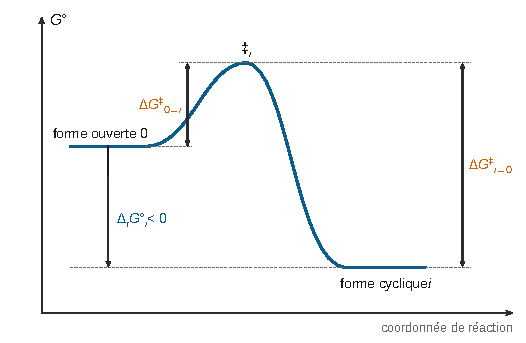
\includegraphics{figures/q5-profil-enthalpie-libre.pdf}
\caption*{Figure 1 --- Profil d'enthalpie libre standard de la cyclisation 0 → i :
les deux sens passent par le même complexe activé ‡i}
\end{figure}

Avec \(\Delta_rG^\circ_i<0\), on a \(k_{i0}<k_{0i}\) : l'ouverture est plus lente que la fermeture.

\hypertarget{question-6}{%
\subsection{Question 6}\label{question-6}}

On admet que \(\Delta_rH^\circ_i\) et \(\Delta_rS^\circ_i\) ne dépendent pas de \(T\) (approximation d'Ellingham), et on écrit \(\Delta_rG^\circ_i=\Delta_rH^\circ_i-T\Delta_rS^\circ_i\) :

\equationajustee{\begin{aligned}
\frac{k_{0i}}{k_{i0}}&=e^{-\frac{\Delta_rG^\circ_i}{RT}}\\
&=\underbrace{e^{\frac{\Delta_rS^\circ_i}{R}}}_{\eta_i}\cdot\underbrace{e^{-\frac{\Delta_rH^\circ_i}{RT}}}_{B_i(T)}
\end{aligned}}

\equationajustee{\boxed{\eta_i=\exp\left(\frac{\Delta_rS^\circ_i}{R}\right)\ \text{(entropique, \text{indépendant} de }T)}}

\equationajustee{\boxed{B_i(T)=\exp\left(-\frac{\Delta_rH^\circ_i}{RT}\right)\ \text{(enthalpique)}}}

\hypertarget{question-7}{%
\subsection{Question 7}\label{question-7}}

Hypothèses :

\begin{enumerate}
\def\labelenumi{\arabic{enumi}.}
\tightlist
\item
  Les deux équilibres de cyclisation sont atteints.
\item
  Les cyclisations sont des actes élémentaires, donc leurs vitesses suivent la loi de Van 't Hoff.
\item
  La solution est idéale et diluée : \(a_i=c_i/c^\circ\).
\item
  \(\Delta_rH^\circ_i\) et \(\Delta_rS^\circ_i\) sont indépendantes de \(T\).
\item
  La forme ouverte est très minoritaire (Q4) : \(c_0\ll c_1,c_2\), donc \(x_1+x_2\simeq1\).
\end{enumerate}

À l'équilibre, les vitesses des deux actes opposés sont égales : \(k_{0i}c_0=k_{i0}c_i\). D'où :

\equationajustee{\frac{c_i}{c_0}=\frac{k_{0i}}{k_{i0}}=\eta_i\,e^{-\frac{\Delta_rH^\circ_i}{RT}}}

\equationajustee{\begin{aligned}
x_i&=\frac{c_i}{c_0+c_1+c_2}\\
&\simeq\frac{c_i}{c_1+c_2}\\
&=\frac{c_i/c_0}{\sum_m c_m/c_0}
\end{aligned}}

D'où :

\equationajustee{\boxed{x_i=\frac{\eta_i\,e^{-\frac{\Delta_rH^\circ_i}{RT}}}{\sum_{m=1}^{2}\eta_m\,e^{-\frac{\Delta_rH^\circ_m}{RT}}}}}

\hypertarget{question-8}{%
\subsection{Question 8}\label{question-8}}

D'après Q7, et puisque \(\eta_2/\eta_1=e^{\Delta_rS^\circ_{1\to2}/R}\) :

\equationajustee{\ln\frac{x_2}{x_1}=\frac{\Delta_rS^\circ_{1\to2}}{R}-\frac{\Delta_rH^\circ_{1\to2}}{R}\cdot\frac1T}

\begin{longtable}[]{@{}
  >{\raggedright\arraybackslash}p{(\columnwidth - 12\tabcolsep) * \real{0.1429}}
  >{\raggedright\arraybackslash}p{(\columnwidth - 12\tabcolsep) * \real{0.1429}}
  >{\raggedright\arraybackslash}p{(\columnwidth - 12\tabcolsep) * \real{0.1429}}
  >{\raggedright\arraybackslash}p{(\columnwidth - 12\tabcolsep) * \real{0.1429}}
  >{\raggedright\arraybackslash}p{(\columnwidth - 12\tabcolsep) * \real{0.1429}}
  >{\raggedright\arraybackslash}p{(\columnwidth - 12\tabcolsep) * \real{0.1429}}
  >{\raggedright\arraybackslash}p{(\columnwidth - 12\tabcolsep) * \real{0.1429}}@{}}
\toprule\noalign{}
\begin{minipage}[b]{\linewidth}\raggedright
\(T\) (K)
\end{minipage} & \begin{minipage}[b]{\linewidth}\raggedright
283
\end{minipage} & \begin{minipage}[b]{\linewidth}\raggedright
298
\end{minipage} & \begin{minipage}[b]{\linewidth}\raggedright
313
\end{minipage} & \begin{minipage}[b]{\linewidth}\raggedright
323
\end{minipage} & \begin{minipage}[b]{\linewidth}\raggedright
358
\end{minipage} & \begin{minipage}[b]{\linewidth}\raggedright
363
\end{minipage} \\
\midrule\noalign{}
\endhead
\bottomrule\noalign{}
\endlastfoot
\(10^3/T\) (K⁻¹) & 3,534 & 3,356 & 3,195 & 3,096 & 2,793 & 2,755 \\
\(x_2/x_1\) & 0,176 & 0,250 & 0,333 & 0,389 & 0,587 & 0,695 \\
\(\ln(x_2/x_1)\) & −1,735 & −1,386 & −1,099 & −0,944 & −0,532 & −0,364 \\
\end{longtable}

La régression linéaire de \(\ln(x_2/x_1)\) en fonction de \(1/T\) donne une pente \(a=-1{,}668\times10^3\) K et une ordonnée à l'origine \(b=4{,}195\). Le coefficient \(R^2=0{,}993\) valide le modèle.

\equationajustee{\begin{aligned}
\Delta_rH^\circ_{1\to2}&=-aR\\
&=1{,}668\times10^3\times8{,}31\\
\Delta_rS^\circ_{1\to2}&=bR\\
&=4{,}195\times8{,}31
\end{aligned}}

\equationajustee{\boxed{\Delta_rH^\circ_{1\to2}=+13{,}9\ \mathrm{kJ\cdot mol^{-1}}}}

\equationajustee{\boxed{\Delta_rS^\circ_{1\to2}=+34{,}9\ \mathrm{J\cdot K^{-1}\cdot mol^{-1}}}}

Le passage pyranose → furanose est endothermique mais entropiquement favorable : le furanose est favorisé à haute température, ce que montre le tableau.

\hypertarget{question-9}{%
\subsection{Question 9}\label{question-9}}

On cherche \(x_1=x_2\), soit \(\ln(x_2/x_1)=0\), soit \(\Delta_rG^\circ_{1\to2}(T_i)=0\) :

\equationajustee{\begin{aligned}
T_i&=\frac{\Delta_rH^\circ_{1\to2}}{\Delta_rS^\circ_{1\to2}}\\
&=\frac{13{,}86\times10^3}{34{,}86}
\end{aligned}}

\equationajustee{\boxed{T_i\approx 3{,}97\times10^{2}\ \mathrm{K}\ (\approx124\ ^\circ\mathrm{C})}}

Cette valeur est extrapolée hors du domaine de mesure (283-363 K) : elle suppose \(\Delta_rH^\circ\) et \(\Delta_rS^\circ\) constantes.

\hypertarget{question-10}{%
\subsection{Question 10}\label{question-10}}

À 298 K :

\equationajustee{\begin{aligned}
\Delta_rG^\circ_{1\to2}&=13{,}86\times10^3-298\times34{,}86\\
&=+3{,}5\ \mathrm{kJ\cdot mol^{-1}}>0
\end{aligned}}

D'où \(x_2/x_1=0{,}25\), ce que confirme le tableau. Comme \(298\ \mathrm K<T_i\), le terme enthalpique l'emporte et la forme pyranose domine. On suppose que la compétition entre cycle à 6 et cycle à 5 garde, pour le glucose, les mêmes signes et ordres de grandeur que pour le ribose, dont il ne diffère que par un \(\mathrm{CH_2OH}\). Sous cette hypothèse :

\textbf{À 298 K, le D-glucose se cyclise préférentiellement sous forme pyranose (cycle à six chaînons), celle de la figure 2.}

\hypertarget{question-11}{%
\subsection{Question 11}\label{question-11}}

Dans le saccharose, la liaison osidique unit les deux carbones anomériques, C1 du glucose et C2 du fructose. C'est un acétal formé à partir de deux hémiacétals. Or chaque ose porte de nombreux hydroxyles nucléophiles, que rien ne distingue dans une condensation non enzymatique : quatre en plus de l'anomérique sur le glucopyranose (C2, C3, C4, C6), trois en plus de l'anomérique sur le fructofuranose (C1, C3, C4, C6). On attend donc :

\begin{itemize}
\tightlist
\item
  des \textbf{régioisomères} du saccharose : C1 du glucose lié à C1, C3, C4 ou C6 du fructose, ou C2 du fructose lié à C2, C3, C4 ou C6 du glucose ;
\item
  des produits d'\textbf{homocondensation} (glucose-glucose, fructose-fructose) ;
\item
  des \textbf{oligomères} : un disaccharide garde des hydroxyles libres et, sauf le saccharose, un hémiacétal ;
\item
  des \textbf{isomères de taille de cycle} : chaque ose peut réagir sous forme pyranose ou furanose ;
\item
  enfin, l'acétalisation est \textbf{renversable} en milieu acide (hydrolyse, partie A-II).
\end{itemize}

\textbf{La condensation directe conduit à un mélange statistique de régioisomères et d'oligomères, avec un faible rendement en saccharose. Une synthèse sélective exigerait des protections et déprotections multiples, coûteuses en étapes et en réactifs.}

\hypertarget{ii-hydrolyse-du-saccharose-le-sucre-inverti}{%
\subsection{II --- Hydrolyse du saccharose : le sucre inverti}\label{ii-hydrolyse-du-saccharose-le-sucre-inverti}}

\hypertarget{question-12}{%
\subsection{Question 12}\label{question-12}}

Le \textbf{pouvoir rotatoire} \(\alpha\) d'une solution est l'angle dont tourne le plan de polarisation d'une lumière polarisée rectilignement qui la traverse. Il est compté positivement vers la droite pour un observateur qui reçoit la lumière (dextrogyre). La loi de Biot l'écrit additivement sur les espèces actives : \(\alpha=\sum_i[\alpha]_i\,\ell\,c_i\), avec \(\ell\) en dm et \(c_i\) concentration massique en g·mL⁻¹.

\emph{Solution initiale} : \(c_S=30/100=0{,}300\ \mathrm{g\cdot mL^{-1}}\).

\equationajustee{\begin{aligned}
\alpha_0&=[\alpha]_S\,\ell\,c_S\\
&=66\times0{,}615\times0{,}300
\end{aligned}}

\equationajustee{\boxed{\alpha_0=+12{,}2^\circ}}

\emph{Temps infini} : l'hydrolyse est quantitative. \(n_0=30/342=8{,}77\times10^{-2}\) mol donne \(n_0\) de glucose et \(n_0\) de fructose, soit \(m_G=m_F=15{,}8\) g dans 100 mL :

\equationajustee{\begin{aligned}
\alpha_\infty&=\ell\,(c_G[\alpha]_G+c_F[\alpha]_F)\\
&=0{,}615\times0{,}158\times(52-92)
\end{aligned}}

\equationajustee{\boxed{\alpha_\infty=-3{,}9^\circ}}

Le signe du pouvoir rotatoire s'inverse au cours de la réaction, d'où le nom de sucre « inverti ».

\hypertarget{question-13}{%
\subsection{Question 13}\label{question-13}}

\begin{itemize}
\tightlist
\item
  \textbf{Acide chlorhydrique} : \(\mathrm{H^+}\) catalyse l'hydrolyse de l'acétal, trop lente sans catalyseur. HCl est un acide fort, donc \([\mathrm{H^+}]\) est connue et reste constante, puisque le catalyseur n'est pas consommé.
\item
  \textbf{Eau solvant, en très large excès} (environ 5,5 mol pour 0,088 mol de saccharose) : sa concentration est constante, l'ordre est dégénéré par rapport à l'eau et \(v=k_{\text{obs}}[S]^p\).
\item
  \textbf{Température fixée (298 K)} : \(k\) dépend de \(T\) (loi d'Arrhenius), et c'est la température à laquelle les pouvoirs rotatoires spécifiques sont donnés (\(\lambda=589{,}3\) nm imposée de même).
\item
  \textbf{Deux solutions ne différant que par \([\mathrm{H^+}]\)} : elles permettent d'accéder à l'ordre par rapport à \(\mathrm{H^+}\).
\item
  \textbf{Polarimétrie} : réactif et produits sont optiquement actifs, avec des \([\alpha]\) très différents et même de signes opposés. \(\alpha\) est additif et varie de \(+12{,}2^\circ\) à \(-3{,}9^\circ\). La mesure est continue, non destructive et ne demande ni prélèvement ni trempe.
\item
  \textbf{Forte concentration en sucre} (30 g pour 100 mL) : elle donne des angles mesurables avec précision.
\end{itemize}

\hypertarget{question-14}{%
\subsection{Question 14}\label{question-14}}

Avec \(V\) le volume de la solution, \(n(S)=n_0-n_s\) et \(n(G)=n(F)=n_s\). La concentration massique vaut \(c_i=n_iM_i/V\) :

\equationajustee{\boxed{\alpha(t)=\frac{\ell}{V}\Big[[\alpha]_S(n_0-n_s)M_S+[\alpha]_G\,n_s\,M_G+[\alpha]_F\,n_s\,M_F\Big]}}

\equationajustee{\boxed{\alpha(0)=\frac{\ell}{V}[\alpha]_S\,n_0\,M_S}}

\equationajustee{\boxed{\alpha(\infty)=\frac{\ell}{V}\,n_0\big([\alpha]_GM_G+[\alpha]_FM_F\big)}}

(\(n_s\to n_0\) puisque la réaction est quantitative.)

\hypertarget{question-15}{%
\subsection{Question 15}\label{question-15}}

Par différence des expressions de Q14 :

\equationajustee{\alpha(t)-\alpha_\infty=\frac{\ell}{V}(n_0-n_s)\big([\alpha]_SM_S-[\alpha]_GM_G-[\alpha]_FM_F\big)}

La parenthèse est positive :

\equationajustee{66\times342-(52-92)\times180=2{,}98\times10^4>0}

Donc \(\alpha-\alpha_\infty\) est proportionnel à \([S]\). Pour un ordre 1 par rapport au saccharose, l'ordre étant dégénéré par rapport à l'eau et \([\mathrm{H^+}]\) constante, \([S]=[S]_0e^{-k_{\text{obs}}t}\), d'où :

\equationajustee{\ln(\alpha-\alpha_\infty)=\ln(\alpha_0-\alpha_\infty)-k_{\text{obs}}\,t}

Avec \(\alpha_\infty=-3{,}88^\circ\) (Q12), pour la solution A :

\begin{longtable}[]{@{}
  >{\raggedright\arraybackslash}p{(\columnwidth - 16\tabcolsep) * \real{0.1111}}
  >{\raggedright\arraybackslash}p{(\columnwidth - 16\tabcolsep) * \real{0.1111}}
  >{\raggedright\arraybackslash}p{(\columnwidth - 16\tabcolsep) * \real{0.1111}}
  >{\raggedright\arraybackslash}p{(\columnwidth - 16\tabcolsep) * \real{0.1111}}
  >{\raggedright\arraybackslash}p{(\columnwidth - 16\tabcolsep) * \real{0.1111}}
  >{\raggedright\arraybackslash}p{(\columnwidth - 16\tabcolsep) * \real{0.1111}}
  >{\raggedright\arraybackslash}p{(\columnwidth - 16\tabcolsep) * \real{0.1111}}
  >{\raggedright\arraybackslash}p{(\columnwidth - 16\tabcolsep) * \real{0.1111}}
  >{\raggedright\arraybackslash}p{(\columnwidth - 16\tabcolsep) * \real{0.1111}}@{}}
\toprule\noalign{}
\begin{minipage}[b]{\linewidth}\raggedright
\(t\) (min)
\end{minipage} & \begin{minipage}[b]{\linewidth}\raggedright
15
\end{minipage} & \begin{minipage}[b]{\linewidth}\raggedright
30
\end{minipage} & \begin{minipage}[b]{\linewidth}\raggedright
45
\end{minipage} & \begin{minipage}[b]{\linewidth}\raggedright
82
\end{minipage} & \begin{minipage}[b]{\linewidth}\raggedright
115
\end{minipage} & \begin{minipage}[b]{\linewidth}\raggedright
177
\end{minipage} & \begin{minipage}[b]{\linewidth}\raggedright
222
\end{minipage} & \begin{minipage}[b]{\linewidth}\raggedright
330
\end{minipage} \\
\midrule\noalign{}
\endhead
\bottomrule\noalign{}
\endlastfoot
\(\alpha\) (°) & 10 & 8,5 & 6,5 & 3,5 & 2 & 0 & −1 & −2,5 \\
\(\alpha-\alpha_\infty\) (°) & 13,88 & 12,38 & 10,38 & 7,38 & 5,88 & 3,88 & 2,88 & 1,38 \\
\(\ln(\alpha-\alpha_\infty)\) & 2,631 & 2,516 & 2,340 & 1,999 & 1,772 & 1,357 & 1,059 & 0,325 \\
\end{longtable}

La régression linéaire donne une pente de \(-7{,}27\times10^{-3}\) min⁻¹, une ordonnée de 2,673 et \(R^2=0{,}995\) : les points sont alignés sans courbure systématique.

\equationajustee{\boxed{\text{ordre partiel 1 par rapport au saccharose, } k_{\text{obs}}^A=7{,}27\times10^{-3}\ \mathrm{min^{-1}}\ (t_{1/2}\approx95\ \mathrm{min})}}

Contrôle : l'ordonnée à l'origine donne \(\alpha_0\approx+10{,}6^\circ\), contre \(+12{,}2^\circ\) calculés. Cet écart de 13 \% s'explique vraisemblablement par un volume réel supérieur à 100 mL (30 g de sucre dissous dans 100 mL d'acide). Il n'affecte pas la pente.

\hypertarget{question-16}{%
\subsection{Question 16}\label{question-16}}

On écrit \(v=k[S][\mathrm{H^+}]^p\), avec \([\mathrm{H^+}]\) constante dans chaque expérience. Donc \(k_{\text{obs}}=k[\mathrm{H^+}]^p\).

Le même traitement qu'en Q15 appliqué à la solution B (\(\ln(\alpha-\alpha_\infty)\) = 2,700 ; 2,631 ; 2,556 ; 2,387 ; 2,184 ; 1,929 ; 1,683 ; 1,357) donne \(k_{\text{obs}}^B=4{,}42\times10^{-3}\) min⁻¹ (\(R^2=0{,}990\)). D'où :

\equationajustee{\begin{aligned}
p&=\frac{\ln(k^A_{\text{obs}}/k^B_{\text{obs}})}{\ln(0{,}92/0{,}53)}\\
&=\frac{\ln1{,}646}{\ln1{,}736}\\
&=\frac{0{,}498}{0{,}551}\\
&=0{,}90
\end{aligned}}

Compte tenu de la précision des mesures (angles à 0,5° près), on retient \(p=1\) :

\equationajustee{\boxed{\text{ordre 1 par rapport \text{à} } \mathrm{H^+}}}

La constante de vitesse s'obtient par \(k=k_{\text{obs}}/[\mathrm{H^+}]\) :

\equationajustee{\begin{aligned}
k_A&=\frac{7{,}27\times10^{-3}}{0{,}92}\\
&=7{,}9\times10^{-3}\ \mathrm{L\cdot mol^{-1}\cdot min^{-1}}\\
k_B&=\frac{4{,}42\times10^{-3}}{0{,}53}\\
&=8{,}3\times10^{-3}\ \mathrm{L\cdot mol^{-1}\cdot min^{-1}}
\end{aligned}}

\equationajustee{\boxed{k\approx8{,}1\times10^{-3}\ \mathrm{L\cdot mol^{-1}\cdot min^{-1}}=1{,}4\times10^{-4}\ \mathrm{L\cdot mol^{-1}\cdot s^{-1}}\ \text{\text{à} 298 K}}}

avec \(v=k[S][\mathrm{H^+}]\). L'ordre par rapport à l'eau reste inconnu, masqué par la dégénérescence.

\begin{center}\rule{0.5\linewidth}{0.5pt}\end{center}

\hypertarget{partie-b-uxe9tude-du-procuxe9duxe9-industriel-du-raffinage-du-sucre-de-betterave}{%
\section{Partie B --- Étude du procédé industriel du raffinage du sucre de betterave}\label{partie-b-uxe9tude-du-procuxe9duxe9-industriel-du-raffinage-du-sucre-de-betterave}}

\hypertarget{i-uxe9tape-dextraction-par-diffusion}{%
\subsection{I --- Étape d'extraction par diffusion}\label{i-uxe9tape-dextraction-par-diffusion}}

\hypertarget{question-17}{%
\subsection{Question 17}\label{question-17}}

À \(T\) et \(P\) fixées, le transfert de \(\mathrm dn>0\) mol de saccharose de l'intérieur (int) vers le jus (ext) fait varier l'enthalpie libre de :

\equationajustee{\mathrm dG=(\mu_{\text{ext}}-\mu_{\text{int}})\,\mathrm dn=RT\ln\frac{c_{\text{ext}}}{c_{\text{int}}}\,\mathrm dn}

avec \(\mu=\mu^\circ+RT\ln(c/c^\circ)\) pour une solution diluée idéale. Le jus d'extraction est initialement pauvre en sucre (\(c_{\text{ext}}<c_{\text{int}}\)), donc \(\mathrm dG<0\) : le transfert est spontané. Il cesse quand les potentiels chimiques sont égaux, c'est-à-dire quand les concentrations le sont.

\textbf{Le saccharose diffuse spontanément du milieu où son potentiel chimique est le plus élevé (la cellule, concentrée) vers celui où il est le plus faible (le jus).} L'eau chaude rend la paroi perméable au saccharose.

\hypertarget{question-18}{%
\subsection{Question 18}\label{question-18}}

L'\textbf{osmose} est le passage spontané du \textbf{solvant} à travers une membrane semi-perméable (perméable au solvant, imperméable au soluté), de la solution la plus diluée vers la plus concentrée. Dans ce sens, le potentiel chimique du solvant diminue, car le soluté abaisse ce potentiel.

La \textbf{pression osmotique} \(\Pi\) d'une solution est la surpression qu'il faut lui appliquer pour annuler le flux de solvant venant du solvant pur, c'est-à-dire pour égaler les potentiels chimiques du solvant de part et d'autre de la membrane.

\begin{figure}[H]
\centering
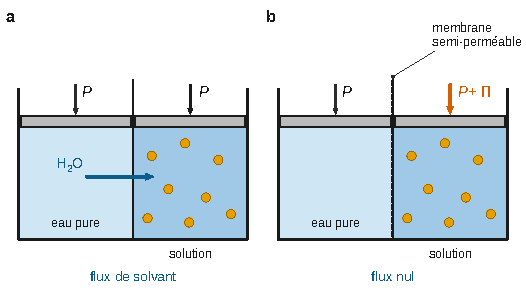
\includegraphics{figures/q18-osmose-pression-osmotique.pdf}
\caption*{Figure 2 --- Osmose : à pressions égales l'eau passe vers la solution
(a) ; une surpression Π sur la solution annule ce flux (b)}
\end{figure}

\hypertarget{question-19}{%
\subsection{Question 19}\label{question-19}}

Hypothèses : membrane strictement semi-perméable, système isotherme ; solution idéale (\(a_{\mathrm{H_2O}}=x(\mathrm{H_2O})\)) ; eau liquide incompressible (\(V^*\) indépendant de \(P\)) ; solution diluée (\(x_S\ll1\), \(n_S\ll n_{\mathrm{H_2O}}\)) ; volume de la solution assimilé à celui de l'eau qu'elle contient.

Comme \(\left(\partial\mu/\partial P\right)_T=V^*\) :

\begin{itemize}
\tightlist
\item
  eau pure à \(P\) : \(\mu=\mu^\circ(\mathrm{H_2O(l)})+V^*(P-P^\circ)\) ;
\item
  eau de la solution à \(P+\Pi\) : \(\mu=\mu^\circ(\mathrm{H_2O(l)})+V^*(P+\Pi-P^\circ)+RT\ln x(\mathrm{H_2O})\).
\end{itemize}

L'équilibre de l'eau impose l'égalité des deux potentiels :

\equationajustee{V^*\Pi=-RT\ln x(\mathrm{H_2O})}

En solution diluée :

\equationajustee{\begin{aligned}
\ln x(\mathrm{H_2O})&=\ln(1-x_S)\\
&\simeq-x_S\\
&\simeq-n_S/n_{\mathrm{H_2O}}
\end{aligned}}

D'où :

\equationajustee{\begin{aligned}
\Pi&\simeq\frac{RT\,n_S}{n_{\mathrm{H_2O}}V^*}\\
&\simeq\frac{RT\,n_S}{V}
\end{aligned}}

\equationajustee{\boxed{\Pi=CRT}}

\hypertarget{question-20}{%
\subsection{Question 20}\label{question-20}}

Un mètre cube de liquide cellulaire a une masse de \(1{,}00\times10^3\) kg (masse volumique de l'eau) et contient 160 kg de saccharose :

\equationajustee{C=\frac{1{,}60\times10^5}{342}=4{,}68\times10^2\ \mathrm{mol\cdot m^{-3}}}

Dans le diffuseur, \(T=343\) K :

\equationajustee{\begin{aligned}
\Pi&=CRT\\
&=4{,}68\times10^2\times8{,}31\times343
\end{aligned}}

\equationajustee{\boxed{\Pi\approx1{,}33\times10^6\ \mathrm{Pa}=13\ \mathrm{bar}}}

On obtient le bon ordre de grandeur, mais 2,5 fois moins que les 34 bar mesurés. Discussion des approximations :

\begin{itemize}
\tightlist
\item
  \textbf{Dilution} : \(x_S=0{,}468/(0{,}468+46{,}7)=1{,}0\times10^{-2}\). La linéarisation \(\ln(1-x_S)\simeq-x_S\) introduit 0,5 \% d'erreur : elle est justifiée.
\item
  \textbf{Volume} : identifier \(n_{\mathrm{H_2O}}V^*\) (0,84 L d'eau par litre de solution) au volume de la solution sous-estime \(\Pi\) d'environ 19 \% (on trouverait 15,9 bar). La masse volumique réelle (environ 1,06 g·mL⁻¹) augmente encore un peu \(C\). Ces effets sont réels mais secondaires.
\item
  \textbf{Idéalité} : à 16 \% en masse, le saccharose, très hydraté, abaisse l'activité de l'eau plus que ne le prévoit sa fraction molaire. \(\Pi\) augmente : l'écart va dans le bon sens.
\item
  \textbf{Seul soluté ?} C'est l'approximation la plus fausse. La pression osmotique est une propriété colligative : elle compte toutes les particules dissoutes. Le jus contient aussi des sels minéraux (K⁺, Na⁺, chlorures\ldots{} qui comptent pour plusieurs particules), des acides organiques et des acides aminés. \textbf{C'est la cause principale de l'écart.}
\end{itemize}

\hypertarget{question-21}{%
\subsection{Question 21}\label{question-21}}

Le jus d'extraction est plus dilué que le suc cellulaire : l'eau entre donc \textbf{dans} les cossettes, en sens inverse du saccharose. Les cossettes se gorgent d'eau et se gonflent ; les cellules peuvent éclater et libérer des impuretés (protéines, pectines, colloïdes). Le transfert du sucre est contrarié, et il faut plus d'eau d'extraction pour épuiser les cossettes.

\textbf{Le problème majeur : il faut beaucoup d'eau pour extraire le sucre, et le jus obtenu est dilué. Toute cette eau devra ensuite être évaporée (partie B-III), ce qui est le poste énergétique le plus lourd du procédé.} Le jus est en outre plus chargé en impuretés. D'où le fonctionnement à contre-courant des diffuseurs, qui limite les écarts de concentration.

\hypertarget{ii-uxe9tape-de-purification-chaulage-et-carbonatation}{%
\subsection{II --- Étape de purification : chaulage et carbonatation}\label{ii-uxe9tape-de-purification-chaulage-et-carbonatation}}

\hypertarget{question-22}{%
\subsection{Question 22}\label{question-22}}

\equationajustee{\boxed{\mathrm{CaCO_3(s)}=\mathrm{CaO(s)}+\mathrm{CO_2(g)}}}

\hypertarget{question-23}{%
\subsection{Question 23}\label{question-23}}

On suppose les solides purs et non miscibles (activité 1), \(\mathrm{CO_2}\) gaz parfait, et \(\Delta_rH^\circ\), \(\Delta_rS^\circ\) indépendantes de \(T\). Alors \(K^\circ=P(\mathrm{CO_2})_{\text{\text{éq}}}/P^\circ\).

\equationajustee{\begin{aligned}
\Delta_rH^\circ&=-635{,}1-393{,}5+1207{,}4\\
&=+178{,}8\ \mathrm{kJ\cdot mol^{-1}}\\
\Delta_rS^\circ&=38{,}1+213{,}7-92{,}9\\
&=+158{,}9\ \mathrm{J\cdot K^{-1}\cdot mol^{-1}}
\end{aligned}}

À 1000 K :

\equationajustee{\begin{aligned}
\Delta_rG^\circ&=178{,}8\times10^3-1000\times158{,}9\\
&=+1{,}99\times10^4\ \mathrm{J\cdot mol^{-1}}\\
K^\circ&=\exp\left(-\frac{1{,}99\times10^4}{8{,}31\times1000}\right)\\
&=9{,}1\times10^{-2}
\end{aligned}}

\equationajustee{\boxed{P(\mathrm{CO_2})_{\text{\text{éq}}}=9{,}1\times10^{-2}\ \mathrm{bar}\approx9\ \mathrm{kPa}\ \text{\text{à} 1000 K}}}

\hypertarget{question-24}{%
\subsection{Question 24}\label{question-24}}

La réaction est endothermique. D'après la loi de Van 't Hoff :

\equationajustee{\frac{\mathrm d\ln K^\circ}{\mathrm dT}=\frac{\Delta_rH^\circ}{RT^2}>0}

Donc \(K^\circ\) croît avec \(T\), et une élévation de température favorise la décomposition.

Le système (deux solides et un gaz) est monovariant. À \(T\) donnée, la décomposition est \textbf{totale} (rupture d'équilibre) dès que la pression partielle de \(\mathrm{CO_2}\) imposée dans le four reste inférieure à \(P_{\text{\text{éq}}}(T)=K^\circ(T)P^\circ\). Sous 1 bar de \(\mathrm{CO_2}\), il faut \(K^\circ>1\) :

\equationajustee{\begin{aligned}
T&>\frac{\Delta_rH^\circ}{\Delta_rS^\circ}\\
&=\frac{178{,}8\times10^3}{158{,}9}\\
&=1{,}13\times10^3\ \mathrm{K}\ (\approx850\ ^\circ\mathrm{C})
\end{aligned}}

\textbf{On travaille au-dessus de 1130 K environ, et d'autant plus bas qu'on évacue le \(\mathrm{CO_2}\).} On ne monte pas au-delà du nécessaire : chaque degré a un coût énergétique (la réaction consomme 178,8 kJ par mole), et une température excessive fritte la chaux, ce qui la rend moins réactive.

\hypertarget{question-25}{%
\subsection{Question 25}\label{question-25}}

\textbf{Première partie (basse température, croissance exponentielle).} \(\mathrm{CaCO_3(s)}\), \(\mathrm{CaO(s)}\) et \(\mathrm{CO_2(g)}\) coexistent à l'équilibre. Il y a 3 constituants, 1 équilibre et 3 phases, d'où la variance :

\equationajustee{v=(3-1)+2-3=1}

\(P\) ne dépend donc que de \(T\) :

\equationajustee{\begin{aligned}
P&=P^\circ K^\circ(T)\\
&=P^\circ\exp\left(-\frac{\Delta_rH^\circ-T\Delta_rS^\circ}{RT}\right)
\end{aligned}}

On passe ainsi de \(4\times10^{-4}\) bar à 800 K à 0,09 bar à 1000 K.

\textbf{Seconde partie (portion affine).} Tout le carbonate a été décomposé. Il reste \(\mathrm{CaO(s)}\) et \(n=1\) mol de \(\mathrm{CO_2}\) dans \(V=150\) L. L'équilibre est rompu, et la pression croît linéairement :

\equationajustee{\begin{aligned}
P&=\frac{nRT}{V}\\
&=5{,}54\times10^{-4}\,T\ \text{(en bar)}
\end{aligned}}

On lit 0,61 bar à 1100 K et 0,66 bar à 1200 K.

La rupture de pente correspond à la disparition du dernier grain de carbonate, quand \(P^\circ K^\circ(T)=nRT/V\).

\hypertarget{question-26}{%
\subsection{Question 26}\label{question-26}}

\begin{lstlisting}[language=Python]
import scipy.optimize as op
from math import exp

# Définition de la fonction donnant la pression pour T < Tchgt
def f(T):
    return exp(-(178.8e3 - T*158.9)/(8.31*T))   # P = K°(T).P° en bar

# Définition de la fonction donnant la pression lorsque T > Tchgt
def g(T):
    return 1*8.31*T/150e-3/1e5                  # P = nRT/V en bar (n = 1 mol, V = 0,150 m3)

# Détermination de Tchgt
def h(T):
    return f(T) - g(T)

print(op.bisect(h, 800, 1200))
\end{lstlisting}

\(h(800)<0\) et \(h(1200)>0\) : la dichotomie s'applique. Le script renvoie \textbf{\(T_{\text{chgt}}\approx1097\) K}, pour \(P\approx0{,}61\) bar, en accord avec la figure 7. Les deux fonctions doivent rendre la pression dans la même unité.

\hypertarget{question-27}{%
\subsection{Question 27}\label{question-27}}

Lectures (temps pour atteindre une conversion totale) :

\begin{longtable}[]{@{}
  >{\raggedright\arraybackslash}p{(\columnwidth - 10\tabcolsep) * \real{0.2926}}
  >{\raggedright\arraybackslash}p{(\columnwidth - 10\tabcolsep) * \real{0.2123}}
  >{\raggedright\arraybackslash}p{(\columnwidth - 10\tabcolsep) * \real{0.1163}}
  >{\raggedright\arraybackslash}p{(\columnwidth - 10\tabcolsep) * \real{0.1163}}
  >{\raggedright\arraybackslash}p{(\columnwidth - 10\tabcolsep) * \real{0.1163}}
  >{\raggedright\arraybackslash}p{(\columnwidth - 10\tabcolsep) * \real{0.1163}}@{}}
\toprule\noalign{}
\begin{minipage}[b]{\linewidth}\raggedright
Figure 8, \(P(\mathrm{CO_2})=16{,}71\) kPa
\end{minipage} & \begin{minipage}[b]{\linewidth}\raggedright
820 °C
\end{minipage} & \begin{minipage}[b]{\linewidth}\raggedright
850 °C
\end{minipage} & \begin{minipage}[b]{\linewidth}\raggedright
860 °C
\end{minipage} & \begin{minipage}[b]{\linewidth}\raggedright
890 °C
\end{minipage} & \begin{minipage}[b]{\linewidth}\raggedright
900 °C
\end{minipage} \\
\midrule\noalign{}
\endhead
\bottomrule\noalign{}
\endlastfoot
\(t\) (s) & \textgreater{} 450 (0,92 à 450 s) & ≈ 370 & ≈ 140 & ≈ 100 & ≈ 75 \\
\end{longtable}

\begin{longtable}[]{@{}
  >{\raggedright\arraybackslash}p{(\columnwidth - 8\tabcolsep) * \real{0.2000}}
  >{\raggedright\arraybackslash}p{(\columnwidth - 8\tabcolsep) * \real{0.2000}}
  >{\raggedright\arraybackslash}p{(\columnwidth - 8\tabcolsep) * \real{0.2000}}
  >{\raggedright\arraybackslash}p{(\columnwidth - 8\tabcolsep) * \real{0.2000}}
  >{\raggedright\arraybackslash}p{(\columnwidth - 8\tabcolsep) * \real{0.2000}}@{}}
\toprule\noalign{}
\begin{minipage}[b]{\linewidth}\raggedright
Figure 9, \(T=890\) °C
\end{minipage} & \begin{minipage}[b]{\linewidth}\raggedright
16,71 kPa
\end{minipage} & \begin{minipage}[b]{\linewidth}\raggedright
27,35 kPa
\end{minipage} & \begin{minipage}[b]{\linewidth}\raggedright
36,47 kPa
\end{minipage} & \begin{minipage}[b]{\linewidth}\raggedright
46,59 kPa
\end{minipage} \\
\midrule\noalign{}
\endhead
\bottomrule\noalign{}
\endlastfoot
\(t\) (s) & ≈ 100 & ≈ 190 & ≈ 550 & \textgreater{} 600 \\
\end{longtable}

\begin{itemize}
\tightlist
\item
  La vitesse \textbf{croît fortement avec \(T\)} : la durée est divisée par environ 6 entre 820 et 900 °C. Le gain devient faible au-delà de 890 °C.
\item
  La vitesse \textbf{décroît fortement quand \(P(\mathrm{CO_2})\) augmente} : multiplier \(P(\mathrm{CO_2})\) par 2,8 multiplie la durée par plus de 5.
\end{itemize}

À 890 °C (1163 K), \(\Delta_rG^\circ=178{,}8\times10^3-1163\times158{,}9=-6{,}0\ \mathrm{kJ\cdot mol^{-1}}\), soit \(P_{\text{\text{éq}}}=e^{6000/(8{,}31\times1163)}=1{,}9\) bar. Toutes les pressions de la figure 9 sont donc très inférieures à \(P_{\text{\text{éq}}}\) : la décomposition est thermodynamiquement totale et le ralentissement est d'origine \textbf{cinétique} (le \(\mathrm{CO_2}\) doit diffuser hors du grain à travers la couche de chaux, et sa présence freine la réaction de surface).

\equationajustee{\boxed{T\approx890\text{-}900\ ^\circ\mathrm{C}\ \text{et}\ P(\mathrm{CO_2})\ \text{la plus faible possible (\text{évacuation}, balayage du four)}}}

Monter plus haut n'apporte qu'un gain marginal, pour un coût énergétique accru et un risque de frittage. Le \(\mathrm{CO_2}\) évacué est valorisé à la carbonatation.

\hypertarget{question-28}{%
\subsection{Question 28}\label{question-28}}

2,5 kg de CaO par mètre cube, soit 2,5 g·L⁻¹, donnent par hydratation complète \(\dfrac{2{,}5}{56{,}1}=4{,}46\times10^{-2}\) mol·L⁻¹ de \(\mathrm{Ca(OH)_2}\), soit \(3{,}30\) g·L⁻¹. C'est plus que la solubilité (1,25 g·L⁻¹) : \textbf{la solution est saturée} et du solide subsiste (lait de chaux).

La solubilité molaire vaut :

\equationajustee{\begin{aligned}
s&=\frac{1{,}25}{74{,}1}\\
&=1{,}69\times10^{-2}\ \mathrm{mol\cdot L^{-1}}
\end{aligned}}

La dissolution s'écrit :

\equationajustee{\mathrm{Ca(OH)_2(s)}=\mathrm{Ca^{2+}}+2\,\mathrm{HO^-}}

D'où :

\equationajustee{\begin{aligned}
[\mathrm{HO^-}]&=2s\\
&=3{,}37\times10^{-2}\ \mathrm{mol\cdot L^{-1}}
\end{aligned}}

Avec \(\mathrm pK_e=14\) (aucune valeur n'est donnée à 318 K) : \(\mathrm{pOH}=1{,}47\) et

\equationajustee{\boxed{\mathrm{pH}=12{,}5}}

C'est le pH visé. \textbf{Les conditions de chaulage conviennent} ; le pH est même tamponné par l'équilibre de solubilité tant que du solide subsiste. (Avec \(\mathrm pK_e\approx13{,}4\) à 45 °C, on trouverait environ 11,9. La cible 12,5 est manifestement exprimée dans l'échelle usuelle à 25 °C.)

\hypertarget{iii-uxe9tape-duxe9vaporation}{%
\subsection{III --- Étape d'évaporation}\label{iii-uxe9tape-duxe9vaporation}}

\hypertarget{question-29}{%
\subsection{Question 29}\label{question-29}}

En régime permanent, sans accumulation :

\begin{itemize}
\tightlist
\item
  bilan global : \(D_A=D_V+D_S\), donc \(D_V=1000-220\), soit \(\boxed{D_V=7{,}80\times10^2\ \mathrm{kg\cdot h^{-1}}}\) ;
\item
  bilan en saccharose (non volatil) : \(D_Ax_A=D_Sx_S\), donc \(x_S=\dfrac{150}{220}=0{,}68\), soit le sirop à 68 \% annoncé.
\end{itemize}

\hypertarget{question-30}{%
\subsection{Question 30}\label{question-30}}

On applique le premier principe en système ouvert, en régime permanent, en négligeant le travail d'agitation et les variations d'énergie cinétique et potentielle : \(\Phi=\sum_{\text{sorties}}D\,h-\sum_{\text{\text{entrées}}}D\,h\). L'évaporateur est isotherme, donc il n'y a pas de terme d'échauffement : seule la vaporisation de \(D_V\) compte.

\equationajustee{\begin{aligned}
\Phi&=D_V\,\Delta H_{\text{vap}}\\
&=780\times2257\\
&=1{,}76\times10^6\ \mathrm{kJ\cdot h^{-1}}
\end{aligned}}

\equationajustee{\boxed{\Phi\approx4{,}89\times10^2\ \mathrm{kW}}}

\hypertarget{question-31}{%
\subsection{Question 31}\label{question-31}}

Sans pertes thermiques, la vapeur de chauffe cède \(\Phi\) :

\equationajustee{\begin{aligned}
D_C&=\frac{\Phi}{2740}\\
&=\frac{1{,}76\times10^6}{2740}
\end{aligned}}

\equationajustee{\boxed{D_C\approx6{,}4\times10^2\ \mathrm{kg\cdot h^{-1}}}}

On évapore 1,2 kg d'eau par kilogramme de vapeur vive.

\hypertarget{question-32}{%
\subsection{Question 32}\label{question-32}}

\emph{Premier effet} : il évapore \(D_{V1}=210\) kg·h⁻¹, ce qui demande \(\Phi_1=210\times2257=4{,}74\times10^5\) kJ·h⁻¹, fourni par la vapeur vive :

\equationajustee{D'_C=\frac{210\times2257}{2740}}

\equationajustee{\boxed{D'_C\approx1{,}73\times10^2\ \mathrm{kg\cdot h^{-1}}}}

\emph{Effets suivants} : on fait les hypothèses suivantes. La vapeur produite par un effet se condense entièrement dans l'échangeur de l'effet suivant, où la pression, donc la température d'ébullition, est plus basse. Elle y cède \(\Delta H_{\text{vap}}\) par kilogramme. Les pertes et les chaleurs sensibles sont négligées, et \(\Delta H_{\text{vap}}\) est le même dans les trois effets. Alors chaque effet évapore la même masse que le précédent : \(D_{V2}=D_{V3}=210\) kg·h⁻¹, soit 630 kg·h⁻¹ au total.

\begin{figure}[H]
\centering
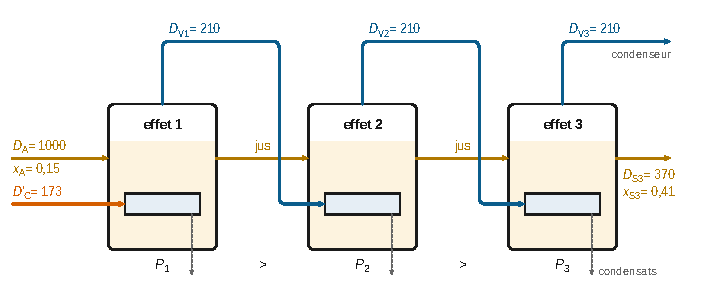
\includegraphics{figures/q32-evaporation-triple-effet.pdf}
\caption*{Figure 3 --- Atelier à triple effet (débits en kg/h) : la vapeur de
chaque effet chauffe l'effet suivant, à pression plus basse}
\end{figure}

Bilans globaux sur l'atelier : \(D_{S3}=1000-630=370\) kg·h⁻¹, et \(D_Ax_A=D_{S3}x_{S3}\) :

\equationajustee{\boxed{x_{S3}=\frac{150}{370}\approx0{,}41\ (41\ \%\ \text{en masse})}}

\emph{Commentaire} : la consommation de vapeur vive est divisée par 3. Il faut 173 kg·h⁻¹ pour évaporer 630 kg·h⁻¹, soit 3,6 kg d'eau par kilogramme de vapeur, contre 1,2 en simple effet. Mais le sirop n'est qu'à 41 \%, loin des 68 \% visés : il faudrait évaporer 779 kg·h⁻¹, soit environ 3,7 effets de 210 kg·h⁻¹. On ajoute donc des effets (« de trois à six »), ou bien on augmente \(D_{V1}\) (260 kg·h⁻¹ par effet, avec \(D'_C\approx214\) kg·h⁻¹). Le multiple effet réutilise la même enthalpie à des températures décroissantes. Les basses températures préservent en outre le saccharose (hydrolyse, caramélisation) ; la contrepartie est un investissement plus lourd.

\hypertarget{iv-analyse-de-puretuxe9}{%
\subsection{IV --- Analyse de pureté}\label{iv-analyse-de-puretuxe9}}

\hypertarget{question-33}{%
\subsection{Question 33}\label{question-33}}

Demi-équations : \(\mathrm{I_2}+2e^-=2\,\mathrm{I^-}\) (\(E^\circ_1=0{,}53\) V) et \(\mathrm{SO_4^{2-}}+4\,\mathrm{H^+}+2e^-=\mathrm{SO_2}+2\,\mathrm{H_2O}\) (\(E^\circ_2=0{,}17\) V).

\equationajustee{\boxed{\mathrm{I_2}+\mathrm{SO_2}+2\,\mathrm{H_2O}\longrightarrow2\,\mathrm{I^-}+\mathrm{SO_4^{2-}}+4\,\mathrm{H^+}}}

\equationajustee{\begin{aligned}
\log K^\circ&=\frac{2(E^\circ_1-E^\circ_2)}{0{,}059}\\
&=\frac{2\times0{,}36}{0{,}059}\\
&=12{,}2
\end{aligned}}

\equationajustee{\boxed{K^\circ\approx1{,}6\times10^{12}}}

La réaction est quantitative, ce qui lui permet de servir de support à un titrage.

\hypertarget{question-34}{%
\subsection{Question 34}\label{question-34}}

Avant l'équivalence, le diiode généré est consommé par l'eau : la solution contient \(\mathrm{I^-}\) mais pas \(\mathrm{I_2}\). Il n'y a pas de branche de réduction de \(\mathrm{I_2}\), et \(-20\ \mu\)A n'est atteint qu'au mur de réduction du solvant : \(\Delta E\) est grand (figure 13).

\textbf{Juste après l'équivalence}, \(\mathrm{I_2}\) en léger excès coexiste avec \(\mathrm{I^-}\). Le couple est rapide, donc la courbe i-E présente une branche d'oxydation de \(\mathrm{I^-}\) et une branche de réduction de \(\mathrm{I_2}\) qui se raccordent sans palier à courant nul au potentiel d'équilibre \(E_{\text{\text{éq}}}\) du couple :

\begin{figure}[H]
\centering
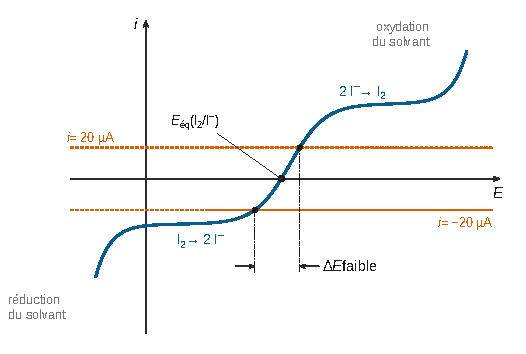
\includegraphics{figures/q34-courbe-ie-apres-equivalence.pdf}
\caption*{Figure 4 --- Courbe courant-potentiel juste après l'équivalence : les
potentiels à ±20 µA encadrent étroitement E\_éq, ΔE est faible}
\end{figure}

Le palier de réduction de \(\mathrm{I_2}\) est petit, car \(\mathrm{I_2}\) est peu abondant, mais il dépasse 20 µA en valeur absolue dès que \(\mathrm{I_2}\) s'accumule un peu. Les deux potentiels correspondant à \(\pm20\ \mu\)A encadrent alors étroitement \(E_{\text{\text{éq}}}\) :

\textbf{La différence de potentiel mesurée chute brutalement à une valeur faible (quelques dizaines de mV au plus) : c'est la détection de l'équivalence (bi-ampérométrie à courant imposé).}

\hypertarget{question-35}{%
\subsection{Question 35}\label{question-35}}

Le diiode est produit à l'anode du générateur (\(2\,\mathrm{I^-}\to\mathrm{I_2}+2e^-\)), donc \(n(\mathrm{I_2})=Q/(2F)\). D'après l'équation de Karl-Fischer, \(\mathrm{H_2O}\) et \(\mathrm{I_2}\) réagissent mole à mole. Avec \(M(\mathrm{H_2O})=18{,}0\) g·mol⁻¹ :

\equationajustee{\begin{aligned}
n(\mathrm{H_2O})&=\frac{0{,}2175}{2\times96\,485}\\
&=1{,}127\times10^{-6}\ \mathrm{mol}\\
m&=2{,}03\times10^{-5}\ \mathrm g
\end{aligned}}

\equationajustee{w=\frac{2{,}029\times10^{-5}}{0{,}1000}}

\equationajustee{\boxed{w=2{,}03\times10^{-4}=0{,}0203\ \%}}

Incertitudes relatives composées quadratiquement (produit et quotient de grandeurs indépendantes) :

\equationajustee{\begin{aligned}
\frac{u(w)}{w}&=\sqrt{\left(\frac{2{,}0\times10^{-3}}{0{,}2175}\right)^2+\left(\frac{1{,}0\times10^{-3}}{0{,}1000}\right)^2}\\
&=1{,}36\times10^{-2}\\
u(w)&=2{,}8\times10^{-4}\ \%
\end{aligned}}

\equationajustee{\begin{aligned}
E_N&=\frac{|w-h|}{\sqrt{u(w)^2+u(h)^2}}\\
&=\frac{0{,}0203-0{,}0200}{\sqrt{(2{,}8\times10^{-4})^2+(1{,}0\times10^{-3})^2}}
\end{aligned}}

\equationajustee{\boxed{E_N\approx0{,}28<2}}

\textbf{La teneur mesurée est compatible avec l'humidité attendue \(h=0{,}020\,\%\).}

\begin{center}\rule{0.5\linewidth}{0.5pt}\end{center}

\hypertarget{partie-c-les-procuxe9duxe9s-uxe9co-responsables-de-lutte-contre-les-nuisibles}{%
\section{Partie C --- Les procédés éco-responsables de lutte contre les nuisibles}\label{partie-c-les-procuxe9duxe9s-uxe9co-responsables-de-lutte-contre-les-nuisibles}}

\hypertarget{i-synthuxe8se-de-la--nuxe9puxe9talactone}{%
\subsection{I --- Synthèse de la (+)-népétalactone}\label{i-synthuxe8se-de-la--nuxe9puxe9talactone}}

\hypertarget{question-36}{%
\subsection{Question 36}\label{question-36}}

(+) signifie que le composé est \textbf{dextrogyre} : il fait tourner le plan de polarisation d'une lumière polarisée rectilignement vers la droite pour un observateur qui reçoit la lumière, autrement dit son pouvoir rotatoire spécifique est positif (à \(\lambda\), \(T\) et solvant donnés). C'est une grandeur expérimentale, sans lien systématique avec les descripteurs \emph{R}/\emph{S} ou D/L.

\hypertarget{question-37}{%
\subsection{Question 37}\label{question-37}}

\emph{Conditions} : \textbf{tétrahydruroborate de sodium \(\mathrm{NaBH_4}\)} dans un solvant protique (éthanol ou méthanol), vers 0 °C puis à température ambiante, puis hydrolyse (eau, acide dilué). \(\mathrm{NaBH_4}\) réduit l'aldéhyde en alcool primaire \textbf{sans toucher à la double liaison C=C} isolée. Le carbone stéréogène n'est pas concerné, donc la configuration \emph{S} est conservée. (On pourrait aussi utiliser \(\mathrm{LiAlH_4}\) dans l'éther anhydre puis une hydrolyse, mais il est inutilement réactif.)

\emph{Mécanisme} (l'ion \(\mathrm{BH_4^-}\) est modélisé comme donneur d'hydrure \(\mathrm{H^-}\)) :

\begin{enumerate}
\def\labelenumi{\arabic{enumi}.}
\tightlist
\item
  \textbf{Addition nucléophile} : le doublet de la liaison B--H attaque le carbone électrophile du carbonyle, et le doublet \(\pi\) de C=O bascule sur l'oxygène. On obtient l'alcoolate \(\mathrm{R{-}CH_2{-}O^-}\) (lié au bore).
\item
  \textbf{Protonation} : un doublet de l'oxygène de l'alcoolate capte le proton de l'alcool solvant (ou de l'eau d'hydrolyse), ce qui donne \(\mathrm{R{-}CH_2OH}\), le (\emph{S})-citronellol.
\end{enumerate}

\equationajustee{\mathrm{R{-}CHO}\xrightarrow{\ \mathrm{H^-}\ (\mathrm{BH_4^-})\ }\mathrm{R{-}CH_2{-}O^-}\xrightarrow{\ \mathrm{EtOH}\ }\mathrm{R{-}CH_2OH}+\mathrm{EtO^-}}

avec \(\mathrm R=-\mathrm{CH_2CH(CH_3)CH_2CH_2CH{=}C(CH_3)_2}\).

\hypertarget{question-38}{%
\subsection{Question 38}\label{question-38}}

Entre le citronellol et les produits \textbf{1} et \textbf{2}, seul change un méthyle terminal porté par la double liaison C=C trisubstituée, c'est-à-dire un méthyle \textbf{allylique}. Il devient \(\mathrm{-CH_2OH}\) (alcool allylique \textbf{2}) ou \(\mathrm{-CHO}\) (énal \textbf{1}). L'alcool primaire, la double liaison et le centre stéréogène sont conservés. Le carbone concerné passe du nombre d'oxydation −III (méthyle) à −I (alcool) puis à +I (aldéhyde).

\textbf{C'est une oxydation allylique (oxydation de Riley) : \(\mathrm{SeO_2}\) catalytique, régénéré par l'hydroperoxyde de \emph{tert}-butyle (oxydant stœchiométrique).} Elle est chimio- et régiosélective : un seul méthyle allylique est oxydé, celui en position \emph{E}.

\hypertarget{question-39}{%
\subsection{Question 39}\label{question-39}}

\emph{Nombre d'oxydation de l'iode dans l'IBX} : l'iode est lié à un carbone aromatique, à un oxygène par une double liaison, à un groupe OH et à l'oxygène du cycle (ester iodé). Chaque liaison avec O donne +I par électron mis en commun (+2 pour I=O, +1 pour I--OH, +1 pour I--O du cycle). La liaison I--C, très peu polarisée, est traitée comme dans les dérivés aryl-iodés usuels (aryle compté comme ligand anionique, +1) :

\equationajustee{\boxed{n.o.(\mathrm I)=+2+1+1+1=+\mathrm V}}

C'est l'iode(V) des λ⁵-iodanes, comme dans l'acide iodique \(\mathrm{HIO_3}\). (Un décompte strict avec l'électronégativité de Pauling, \(\chi_{\mathrm I}=2{,}66>\chi_{\mathrm C}=2{,}55\), donne +III. L'argument reste le même.) Ce nombre d'oxydation est très élevé pour un halogène, dont les états stables sont −I et 0 : l'IBX capte des électrons, c'est un \textbf{oxydant}. Il est réduit en acide 2-iodosobenzoïque (IBA, iode +III dans la même convention) par un échange de 2 électrons, juste ce qu'il faut pour oxyder un alcool primaire en aldéhyde. L'IBA, insoluble dans l'acétonitrile, est éliminé par filtration.

\emph{Oxydant non sélectif (NaClO)} : l'oxydation de l'alcool primaire ne s'arrête pas à l'aldéhyde mais va jusqu'à l'acide carboxylique, et l'aldéhyde conjugué de \textbf{1} est lui aussi oxydé en acide. On obtient le \textbf{diacide} :

\equationajustee{\mathrm{HOOC{-}CH_2{-}CH(CH_3){-}CH_2{-}CH_2{-}CH{=}C(CH_3){-}COOH}}

soit l'acide (\emph{E})-\allowbreak{}2,6-\allowbreak{}diméthyloct-\allowbreak{}2-\allowbreak{}ènedioïque. La double liaison et sa géométrie \emph{E} sont conservées, ainsi que la disposition spatiale autour du carbone stéréogène.

\hypertarget{question-40}{%
\subsection{Question 40}\label{question-40}}

On numérote le 8-oxocitronellal \textbf{3} de C1 (aldéhyde saturé, \(\mathrm{-CH_2{-}CHO}\)) à C8 (aldéhyde conjugué) : \(\mathrm{OHC^1{-}C^2H_2{-}C^3H(CH_3){-}C^4H_2{-}C^5H_2{-}C^6H{=}C^7(CH_3){-}C^8HO}\).

La DIPEA est une base encombrée, non nucléophile. Elle arrache le proton le plus acide utilisable, un proton en \textbf{α du carbonyle saturé (C2)}. On obtient l'\textbf{énolate} :

\equationajustee{\begin{aligned}{}&\mathrm{^-O{-}C^1H{=}C^2H{-}C^3H(CH_3){-}CH_2{-}CH_2{-}CH{=}C(CH_3){-}CHO}\\
\longleftrightarrow\ &\mathrm{O{=}C^1H{-}C^2H^-{-}\cdots}
\end{aligned}}

La charge est délocalisée sur O et sur C2 (mésomérie). Cet énolate est nucléophile en C2.

Justification du choix :

\begin{itemize}
\tightlist
\item
  Les hydrogènes en α de C1 sont acides (\(\mathrm pK_a\approx17\)) parce que l'anion formé est stabilisé par mésomérie avec C=O.
\item
  L'énal n'a pas d'hydrogène en α : C7 ne porte pas d'hydrogène, et l'hydrogène de C8 est aldéhydique. Une déprotonation vinylogue (en γ, sur C5 ou sur le méthyle de C7) donnerait un diénolate qui ne peut pas s'additionner sur son propre système conjugué.
\item
  Seul l'énolate en C2 peut attaquer le carbone β de l'énal (C6) en fermant un cycle \textbf{à cinq chaînons} (C2, C3, C4, C5, C6), celui du squelette de la népétalactone.
\end{itemize}

La DIPEA (\(\mathrm pK_a\approx11\) pour son acide conjugué) ne forme l'énolate qu'en faible quantité. L'addition de Michael qui suit le consomme et déplace l'équilibre, ce qui explique qu'une quantité catalytique de base suffise.

\hypertarget{question-41}{%
\subsection{Question 41}\label{question-41}}

L'accepteur de Michael est l'énal \(\mathrm{C^6H{=}C^7(CH_3){-}C^8H{=}O}\). Son carbone β (C6) est électrophile : la forme mésomère \(\mathrm{^+C^6H{-}C^7(CH_3){=}C^8H{-}O^-}\) le montre, et c'est aussi sur C6 que la BV du système conjugué a son plus gros coefficient. Trois flèches simultanées :

\begin{enumerate}
\def\labelenumi{\arabic{enumi}.}
\tightlist
\item
  le doublet \(\pi\) C1=C2 de l'énolate attaque C6, ce qui forme la liaison C2--C6 et ferme le cyclopentane (le doublet de O⁻ se replie en même temps pour reformer C1=O) ;
\item
  le doublet \(\pi\) C6=C7 se déplace sur la liaison C7--C8 ;
\item
  le doublet \(\pi\) C8=O se replie sur l'oxygène.
\end{enumerate}

\textbf{Second intermédiaire anionique} : un cyclopentane (C2 à C6) qui porte sur C2 le groupe \(\mathrm{-CHO}\) (C1), sur C3 le méthyle, et sur C6 l'énolate \(\mathrm{-C^7(CH_3){=}C^8H{-}O^-}\) ; C2, C3 et C6 sont contigus. Le squelette est celui de la népétalactone. La lactone se ferme ensuite entre l'oxygène de l'énolate et C1, activé en acylazolium par le NHC et l'oxydant A.

\hypertarget{question-42}{%
\subsection{Question 42}\label{question-42}}

\emph{Étalonnage (figure 19)} : le mélange est racémique avec \(C_{\text{tot}}=1\) mmol·L⁻¹, donc \(C_1=C_2=0{,}500\) mmol·L⁻¹ :

\equationajustee{\begin{aligned}
k_1&=\frac{50{,}18}{0{,}500}\\
k_2&=\frac{49{,}82}{0{,}500}
\end{aligned}}

\equationajustee{\boxed{k_1=100{,}4\ \%\cdot\mathrm{L\cdot mmol^{-1}}}}

\equationajustee{\boxed{k_2=99{,}6\ \%\cdot\mathrm{L\cdot mmol^{-1}}}}

\emph{Produit de synthèse (figure 20)} : le pic à 21,98 min est celui de la (+)-népétalactone, puisqu'il a le même temps de rétention que le pic 1 de la figure 19. On calcule les concentrations à un facteur commun près :

\equationajustee{\begin{aligned}
C_1&\propto\frac{98{,}50}{100{,}4}=0{,}981\\
C_2&\propto\frac{1{,}50}{99{,}6}=0{,}0151
\end{aligned}}

\equationajustee{\begin{aligned}
ee&=\frac{|C_1-C_2|}{C_1+C_2}\\
&=\frac{0{,}981-0{,}0151}{0{,}981+0{,}0151}
\end{aligned}}

\equationajustee{\boxed{ee\approx97{,}0\ \%\ \text{en faveur de la (+)-\text{népétalactone}}}}

Comme \(k_1\simeq k_2\) (à 0,7 \% près), le calcul direct sur les aires donne la même valeur.

\hypertarget{question-43}{%
\subsection{Question 43}\label{question-43}}

Trois étapes à partir du (\emph{S})-citronellol : oxydation allylique (70 \%), oxydation par l'IBX (58 \%) et cyclisation NHC (84 \%). Les rendements se multiplient :

\equationajustee{\rho=0{,}70\times0{,}58\times0{,}84}

\equationajustee{\boxed{\rho_{\text{global}}\approx0{,}34=34\ \%}}

\hypertarget{ii-uxe9tude-de-la-phuxe9romone-du-puceron-vert}{%
\subsection{II --- Étude de la phéromone du puceron vert}\label{ii-uxe9tude-de-la-phuxe9romone-du-puceron-vert}}

\hypertarget{question-44}{%
\subsection{Question 44}\label{question-44}}

Le trans-β-farnésène, \(\mathrm{C_{15}H_{24}}\), a quinze carbones, soit trois unités en \(\mathrm C_5\). Sa formule semi-développée est

\equationajustee{\begin{aligned}{}&\mathrm{CH_2{=}CH{-}C({=}CH_2){-}CH_2}\\
\big|\ &\mathrm{CH_2{-}CH{=}C(CH_3){-}CH_2}\\
\big|\ &\mathrm{CH_2{-}CH{=}C(CH_3){-}CH_3}
\end{aligned}}

On numérote la chaîne principale de C1 (extrémité vinylique) à C12. Les ramifications sont sur C3 (méthylidène), C7 et C11 (méthyles). Les coupures entre C4 et C5 et entre C8 et C9 (traits verticaux ci-dessus) font apparaître trois motifs, formés chacun de quatre carbones en chaîne et d'une ramification \(\mathrm C_1\) sur le deuxième carbone. C'est le squelette de l'isoprène \(\mathrm{CH_2{=}C(CH_3){-}CH{=}CH_2}\) (2-méthylbutane).

\begin{lstlisting}
  unité 1              unité 2                 unité 3
  CH2=CH-C(=CH2)-CH2 | CH2-CH=C(CH3)-CH2 |  CH2-CH=C(CH3)-CH3
\end{lstlisting}

Les unités sont enchaînées \textbf{tête-à-queue}. Seul le squelette carboné de chaque isoprène est conservé : les doubles liaisons se sont déplacées lors de l'oligomérisation. \textbf{Le farnésène est un trimère (sesquiterpène) de l'isoprène.}

\hypertarget{question-45}{%
\subsection{Question 45}\label{question-45}}

\emph{Symétrie} : l'allyle est dans le plan \(xy\) et le métal s'approche selon \(z\).

D'après la figure 22, les deux carbones terminaux sont symétriques par rapport au plan \((xOz)\), de part et d'autre selon \(\pm y\), et le carbone central est décalé selon \(x\). Le système \(\pi\) est formé des orbitales \(2p_z\). L'élément de symétrie commun aux deux fragments est le plan \(\sigma=(xOz)\).

\begin{longtable}[]{@{}
  >{\raggedright\arraybackslash}p{(\columnwidth - 2\tabcolsep) * \real{0.6012}}
  >{\raggedright\arraybackslash}p{(\columnwidth - 2\tabcolsep) * \real{0.3688}}@{}}
\toprule\noalign{}
\begin{minipage}[b]{\linewidth}\raggedright
Orbitale
\end{minipage} & \begin{minipage}[b]{\linewidth}\raggedright
Comportement par \(\sigma\) (\(y\to-y\))
\end{minipage} \\
\midrule\noalign{}
\endhead
\bottomrule\noalign{}
\endlastfoot
HO du ligand, \(\psi_2\) (coefficient nul au centre, coefficients opposés aux extrémités) & antisymétrique \\
BV du ligand, \(\psi_3\) (extrémités de même signe, centre de signe opposé) & symétrique \\
\(d_{yz}\) & antisymétrique \\
\(d_{xz}\) & symétrique \\
\end{longtable}

Deux orbitales n'interagissent que si elles ont la même symétrie (recouvrement non nul) :

\equationajustee{\boxed{\mathrm{HO}\ (\psi_2)\longleftrightarrow d_{yz}\qquad\text{et}\qquad \mathrm{BV}\ (\psi_3)\longleftrightarrow d_{xz}}}

Ce sont exactement les corrélations tracées sur la figure 22. Chaque interaction donne une OM liante et une OM antiliante. Par énergie croissante : liante \(d_{yz}/\psi_2\) (surtout ligand), liante \(d_{xz}/\psi_3\) (surtout métal), antiliante \(d_{yz}/\psi_2\) (surtout métal), antiliante \(d_{xz}/\psi_3\) (surtout ligand).

\emph{Occupation} : le ligand est l'anion allyle, dont le système \(\pi\) compte 4 électrons (\(\psi_1^2\psi_2^2\)) : la HO est doublement occupée et la BV vacante. Le métal apporte 2 électrons dans \(d_{xz}\), \(d_{yz}\) étant vide. Ces 4 électrons occupent \textbf{les deux OM liantes}, et les deux antiliantes restent vides. Le bilan est stabilisant :

\begin{itemize}
\tightlist
\item
  \textbf{donation} ligand → métal : \(\psi_2\) (2 e⁻) se mélange à \(d_{yz}\) vide ;
\item
  \textbf{rétrodonation} métal → ligand : \(d_{xz}\) (2 e⁻) se mélange à \(\psi_3\) vide.
\end{itemize}

\hypertarget{question-46}{%
\subsection{Question 46}\label{question-46}}

\begin{itemize}
\tightlist
\item
  Par la donation, le doublet de \(\psi_2\), localisé sur les \textbf{carbones terminaux} et responsable du caractère carbanionique de l'allyle libre, est partagé avec le métal. Il se trouve dans une OM plus basse que la HO de départ. La densité électronique des carbones terminaux diminue : \textbf{le ligand perd son caractère nucléophile et basique}.
\item
  La BV du complexe est l'antiliante \(d_{yz}/\psi_2\). Elle est plus basse que la BV de l'allyle libre et garde des coefficients sur les carbones terminaux : ceux-ci deviennent \textbf{électrophiles}.
\item
  La rétrodonation peuple partiellement \(\psi_3\), antiliante entre carbones voisins : les liaisons C--C de l'allyle sont affaiblies et le ligand est activé.
\end{itemize}

\equationajustee{\boxed{\text{La coordination inverse la \text{réactivité} de l'allyle : de \text{nucléophile} (carbanion libre), il devient \text{électrophile} sur ses carbones terminaux.}}}

Le ligand est stabilisé (« apprivoisé ») tout en restant activé pour les étapes d'insertion du cycle catalytique.

\hypertarget{question-47}{%
\subsection{Question 47}\label{question-47}}

\begin{longtable}[]{@{}
  >{\raggedright\arraybackslash}p{(\columnwidth - 4\tabcolsep) * \real{0.1180}}
  >{\raggedright\arraybackslash}p{(\columnwidth - 4\tabcolsep) * \real{0.3541}}
  >{\raggedright\arraybackslash}p{(\columnwidth - 4\tabcolsep) * \real{0.4979}}@{}}
\toprule\noalign{}
\begin{minipage}[b]{\linewidth}\raggedright
Étape
\end{minipage} & \begin{minipage}[b]{\linewidth}\raggedright
Nom
\end{minipage} & \begin{minipage}[b]{\linewidth}\raggedright
Description
\end{minipage} \\
\midrule\noalign{}
\endhead
\bottomrule\noalign{}
\endlastfoot
1 & Coordination (complexation η²) & l'éthylène se lie au nickel par sa liaison \(\pi\) \\
2 & Insertion migratoire 1,2 & l'alcène s'insère dans la liaison Ni--H, ce qui donne {[}Ni{]}--CH₂CH₃ \\
3 & Coordination & une seconde molécule d'éthylène se coordine \\
4 & Insertion migratoire 1,2 & insertion dans la liaison Ni--C, ce qui donne {[}Ni{]}--CH₂CH₂CH₂CH₃ (croissance de chaîne) \\
5 & β-élimination d'hydrure (puis décoordination) & un H du carbone β passe sur le nickel : libération du but-1-ène et régénération de {[}Ni{]}--H \\
\end{longtable}

{[}Ni{]}--H est régénéré : c'est le catalyseur. La somme des étapes donne :

\equationajustee{\boxed{2\ \mathrm{CH_2{=}CH_2}\xrightarrow{\ [\mathrm{Ni}]{-}\mathrm H\ }\mathrm{CH_2{=}CH{-}CH_2{-}CH_3}\ \ (\text{but-1-\text{ène}})}}

\hypertarget{question-48}{%
\subsection{Question 48}\label{question-48}}

Pour l'éthylène, symétrique, aucune question de régiosélectivité ne se pose. L'isoprène est un diène \textbf{dissymétrique} : à chaque \textbf{insertion migratoire} (étapes 2 et 4), il peut se lier au métal ou à la chaîne par l'une ou l'autre de ses extrémités, en 1,2, 2,1, 1,4 ou 4,1. L'insertion d'un diène dans la liaison Ni--C (ou Ni--H) donne un intermédiaire \textbf{η³-allyle}, le ligand étudié aux Q45 et Q46. La position de la liaison C--C suivante et la géométrie \emph{trans} de la double liaison formée dépendent de la façon dont cet allyle (syn ou anti) réagit, ce que règlent les ligands \(\mathrm{OR}\) et \(\mathrm{PPh(NEt_2)_2}\).

\equationajustee{\boxed{\text{L'\text{étape} \text{clé} est l'insertion migratoire de l'\text{isoprène} (via l'\text{intermédiaire} } \eta^3\text{-allyle) : elle impose l'\text{enchaînement} \text{tête}-\text{à}-queue et la \text{géométrie} } trans.}}

La β-élimination joue un rôle complémentaire. Sa compétition avec une troisième insertion fixe la taille du produit : β-élimination précoce, dimères ; après trois insertions, trimère. L'hydrogène éliminé fixe la position des doubles liaisons terminales : motif \(\mathrm{CH_2{=}CH{-}C({=}CH_2){-}}\) du β-farnésène plutôt que celui de l'α-farnésène.

\end{document}
